% Build from this directory:
% latexmk -norc -pdf -interaction=nonstopmode -halt-on-error -file-line-error lecture05.tex
% Mathematical formalizations and diagrams are original lecture material.
\documentclass[11pt,aspectratio=169]{beamer}
\usepackage[T1]{fontenc}
\usepackage{lmodern,amsmath,amssymb,mathtools,booktabs,array}
\usepackage{tikz}
\usetikzlibrary{arrows.meta,positioning,calc,fit}
\usepackage{listings}
\usepackage{appendixnumberbeamer}

\definecolor{ink}{HTML}{17324D}
\definecolor{accent}{HTML}{006D77}
\definecolor{warm}{HTML}{A74420}
\definecolor{muted}{HTML}{566575}
\definecolor{pale}{HTML}{EDF4F5}
\setbeamercolor{normal text}{fg=ink,bg=white}
\setbeamercolor{structure}{fg=accent}
\setbeamercolor{frametitle}{fg=ink}
\setbeamercolor{alerted text}{fg=warm}
\setbeamercolor{block title}{fg=accent,bg=white}
\setbeamercolor{block body}{fg=ink,bg=white}
\setbeamerfont{frametitle}{size=\Large,series=\bfseries}
\setbeamerfont{title}{size=\LARGE,series=\bfseries}
\setbeamertemplate{navigation symbols}{}
\setbeamertemplate{itemize item}{\color{accent}\small\textbullet}
\setbeamertemplate{theorems}[numbered]
\setbeamersize{text margin left=9mm,text margin right=9mm}
\setbeamertemplate{footline}{\hfill\usebeamercolor[fg]{normal text}%
  \scriptsize\insertframenumber\hspace{9mm}\vspace{3mm}}
\setbeamertemplate{frametitle}{\vspace{3mm}\insertframetitle\par\vspace{2mm}}
\setlength{\parskip}{6pt}
\hypersetup{colorlinks=true,urlcolor=accent,linkcolor=accent,
  pdftitle={Lecture 5: Learning reusable computation},pdfauthor={Csaba Szepesvari}}
\pdfstringdefDisableCommands{\def\translate#1{#1}}

\newcommand{\E}{\mathbb E}
\renewcommand{\P}{\mathbb P}
\newcommand{\R}{\mathbb R}
\newcommand{\N}{\mathbb N}
\newcommand{\Z}{\mathbb Z}
\newcommand{\cC}{\mathcal C}
\newcommand{\cO}{\mathcal O}
\newcommand{\cV}{\mathcal V}
\newcommand{\cA}{\mathcal A}
\newcommand{\cF}{\mathcal F}
\newcommand{\cQ}{\mathcal Q}
\newcommand{\enc}{\operatorname{enc}}
\newcommand{\Read}{\operatorname{Read}}
\newcommand{\Update}{\operatorname{Update}}
\newcommand{\Step}{\operatorname{Step}}
\newcommand{\Run}{\operatorname{Run}}
\newcommand{\unit}{\mathsf{unit}}
\newcommand{\true}{\mathsf{true}}
\newcommand{\false}{\mathsf{false}}
\newcommand{\fail}{\mathsf{fail}}
\newcommand{\halt}{\mathsf{halt}}
\newcommand{\op}[1]{\mathsf{#1}}
\newcommand{\call}{\texttt{[call]}}
\newcommand{\ret}{\texttt{[ret]}}
\newcommand{\cfg}[4]{\langle #1,#2,#3,#4\rangle}
\newcommand{\source}[1]{\par\vfill{\scriptsize\color{muted}#1\par}}
\newcommand{\point}[1]{\par\medskip{\color{accent}\bfseries #1}\par}
\newcommand{\schsource}{\source{Schuurmans (2023), Sections 2--5.}}
\newcommand{\micsource}{\source{Xu et al. (2026), Sections 2--3.}}
\newcommand{\backref}[2]{\hfill\hyperlink{#1}{\scriptsize #2 $\rightarrow$}}
\newtheorem{proposition}{Proposition}
\newtheorem{definitionx}{Definition}
\tikzset{box/.style={draw=accent,thick,minimum height=10mm,align=center,
  inner sep=5pt},arr/.style={-{Stealth[length=2mm]},thick,draw=accent},
  cell/.style={draw=ink,minimum width=10mm,minimum height=9mm,inner sep=1pt},
  smalllabel/.style={font=\small,text=muted,align=center}}
\lstset{basicstyle=\ttfamily\small,columns=fullflexible,keepspaces=true,
  showstringspaces=false,keywordstyle=\color{accent}\bfseries,
  morekeywords={if,then,else,return,result,def},commentstyle=\color{muted}}

\title{Learning reusable computation}
\subtitle{Lecture 5 --- Mathematical Foundations of Modern AI}
\author{Csaba Szepesv\'ari}
\date{}

\begin{document}

\begin{frame}[plain]
\vspace{12mm}
{\usebeamerfont{title}\color{ink}\inserttitle\par}
\vspace{5mm}
{\large\insertsubtitle\par}
\vspace{12mm}
\textbf{How can one next-token predictor execute many different programs?}
\vspace{8mm}

Neural controller with external memory\par
Scaffolded neural interpreter\par
Self-contained neural interpreter
\vfill
{\small Dale Schuurmans (2023)\quad\textbullet\quad Ruize Xu et al. (2026)}
\end{frame}

\begin{frame}{What could prediction teach a model to do?}
Lectures 3--4: next-token log loss fits a distribution over sequences.
\[
  -\log q_\theta(x_{1:T})
  =\sum_{t=1}^T-\log q_\theta(x_t\mid x_{<t}).
\]
Suppose the sequences describe computations, with successive states
\[
  \sigma_0\ \longmapsto\ \sigma_1\ \longmapsto\ \cdots\ \longmapsto\ \sigma_L.
\]
\point{The same transition rule can appear in many different tasks.}
Today: specify that rule, expose it in training data, and ask whether a
transformer learns to apply it in new computations.
\end{frame}

\begin{frame}{A name lets us reuse a definition}
Once a procedure has a name, later instructions can refer to its body:
\[
  \Delta(\mathtt{twice})=(x,\,\mathtt{step}(\mathtt{step}(x))).
\]
\begin{center}
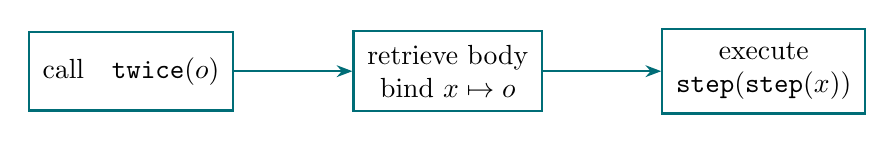
\begin{tikzpicture}[node distance=15mm]
\node[box] (name) {call\quad$\mathtt{twice}(o)$};
\node[box,right=of name] (bind) {retrieve body\\bind $x\mapsto o$};
\node[box,right=of bind] (body) {execute\\$\mathtt{step}(\mathtt{step}(x))$};
\draw[arr] (name)--(bind);
\draw[arr] (bind)--(body);
\end{tikzpicture}
\end{center}
The model must connect a symbol to its definition, preserve bindings, and
resume the caller after the procedure finishes.

\point{Can predictive training recover these reusable operations?}
\end{frame}

\begin{frame}{The target is a shared interpreter}
Fix a deterministic decoder. Let $p$ be a program and $x$ its input.
\begin{definitionx}[Exact execution]
A system with fixed neural parameters $\theta$ executes a program family if
\[
  \Run_\theta(p,x)\simeq p(x)
  \qquad\text{for every allowed }(p,x).
\]
Here $\simeq$ means the same returned value, or divergence on both sides.
\end{definitionx}
The run may use many model calls and writable memory. The system is
\emph{universal} when it executes an effective encoding of every Turing machine.
\point{Different programs; the same learned execution mechanism.}
\end{frame}

\begin{frame}{Universality and learned execution}
We will compare three ways to divide the execution between a neural model
and its surrounding system.

\small
\begin{tabular}{@{}>{\raggedright\arraybackslash}p{.40\textwidth}
  >{\raggedright\arraybackslash}p{.55\textwidth}@{}}
\toprule
Our name & Execution mechanism\\
\midrule
Neural controller with external memory &
External code supplies operands and applies the selected commands.\\[7pt]
Scaffolded neural interpreter &
The model retrieves and updates language state. A fixed scaffold contracts calls.\\[7pt]
Self-contained neural interpreter &
One continuous generation executes the program, with intermediate tokens or directly.\\
\bottomrule
\end{tabular}
\normalsize

\textbf{Universality:} can the whole system execute arbitrary computations?

\textbf{Learning:} how much of the execution mechanism can the model learn?
\end{frame}

\section{Neural controller with external memory}

\begin{frame}{Schuurmans: 29 local cases suffice}
A fixed universal Turing machine has 15 control states and 2 tape symbols.
Schuurmans implements its controller through \alert{29 distinct LLM prompts}.

\begin{center}
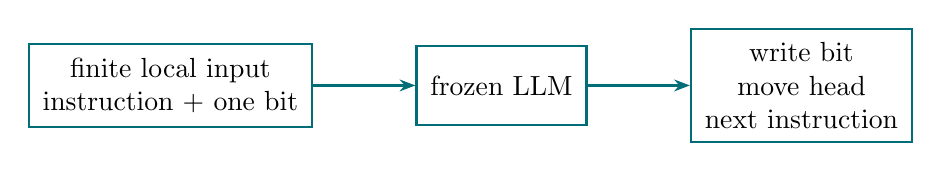
\begin{tikzpicture}[node distance=13mm]
\node[box] (local) {finite local input\\instruction + one bit};
\node[box,right=of local] (model) {frozen LLM};
\node[box,right=of model] (action) {write bit\\move head\\next instruction};
\draw[arr] (local)--(model);
\draw[arr] (model)--(action);
\end{tikzpicture}
\end{center}
The paper prints Flan-U-PaLM 540B's greedy responses for all 29 prompts.
The tape is stored externally.

\point{Why can checking a finite table certify arbitrarily long computations?}
\source{Schuurmans (2023), Sections 2--5. A sign discrepancy between its table
and printed prompt program is documented in backup.}
\end{frame}

\begin{frame}{A Turing machine changes one tape cell at a time}
Let $\cQ$ be a finite set of control states and $\Sigma$ a finite tape alphabet.
An instruction is
\[
 \delta(q,b)=(b',d,q'),\quad d\in\{-1,+1\},
 \qquad\text{or}\qquad\delta(q,b)=\halt.
\]
A \emph{configuration} is $\sigma=(q,i,\tau)$, where $i\in\Z$ is the head
position and $\tau:\Z\to\Sigma$ is blank outside a finite set.
\[
  (q,i,\tau)\longmapsto
  \bigl(q',\ i+d,\ \tau[i\mapsto b']\bigr),
  \qquad (b',d,q')=\delta(q,\tau(i)).
\]
\begin{center}
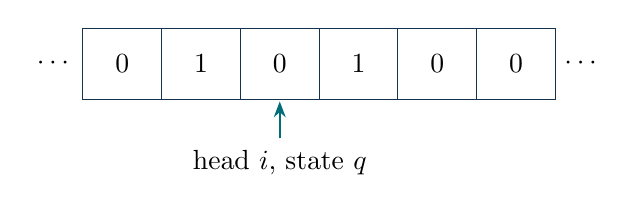
\begin{tikzpicture}
\foreach \x/\v in {0/0,1/1,2/0,3/1,4/0,5/0}
  \node[cell] at (\x,0) {$\v$};
\node at (-.85,0) {$\cdots$}; \node at (5.85,0) {$\cdots$};
\draw[arr] (2,-.95)--(2,-.48);
\node[anchor=north] at (2,-.98) {head $i$, state $q$};
\end{tikzpicture}
\end{center}
\end{frame}

\begin{frame}{The external code resolves the memory addresses}
\begin{center}
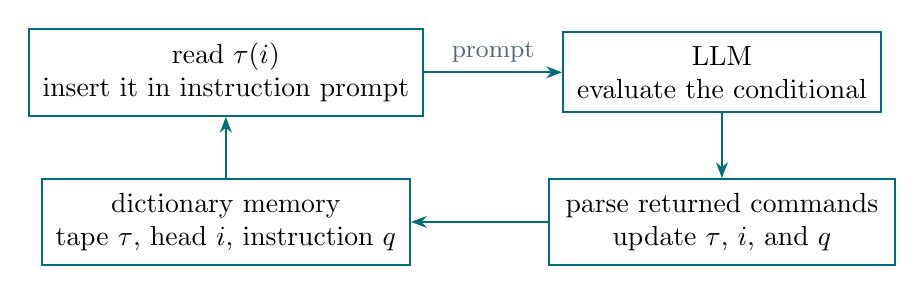
\begin{tikzpicture}
\node[box,minimum width=4.4cm] (mem) at (0,0)
  {dictionary memory\\tape $\tau$, head $i$, instruction $q$};
\node[box,minimum width=3.5cm] (read) at (0,1.9)
  {read $\tau(i)$\\insert it in instruction prompt};
\node[box,minimum width=3.5cm] (llm) at (6.3,1.9)
  {LLM\\evaluate the conditional};
\node[box,minimum width=4.4cm] (write) at (6.3,0)
  {parse returned commands\\update $\tau$, $i$, and $q$};
\draw[arr] (mem)--(read);
\draw[arr] (read)--node[above,smalllabel]{prompt}(llm);
\draw[arr] (llm)--(write);
\draw[arr] (write)--(mem);
\end{tikzpicture}
\end{center}
The head address and the rest of the tape stay outside the neural input.

\point{Longer computations require more cycles and possibly more tape.}
The neural controller continues to receive the same finite set of inputs.
\schsource
\end{frame}

\begin{frame}[fragile]{One prompt implements one conditional instruction}
For control state $A$:
\[
 \delta(A,0)=(0,+1,B),\qquad \delta(A,1)=(1,+1,A).
\]
\begin{columns}[T,onlytextwidth]
\begin{column}{.51\textwidth}
\textbf{Prompt after reading the tape}
\begin{lstlisting}
result = (write 0, right, state B)
if 1 == 1:
    result = (write 1, right, state A)
return result
\end{lstlisting}
\end{column}
\begin{column}{.45\textwidth}
\textbf{Parsed result}
\[
 (b',d,q')=(1,+1,A).
\]
The external code writes $1$ at the current address and increments the address.
\end{column}
\end{columns}
\point{The model selects commands; the memory implementation applies them.}
\source{Simplified notation for Schuurmans's prompt program, Section 4.
The original returns assignment strings with memory-substitution markers.}
\end{frame}

\begin{frame}{Correct local transitions give correct full executions}
Let $N_\theta(q,b)$ be the parsed neural response, and define
\[
 \Step_\theta(q,i,\tau)
 =\Update\bigl((q,i,\tau),N_\theta(q,\tau(i))\bigr).
\]
\begin{proposition}[Exact simulation]
If $N_\theta(q,b)=\delta(q,b)$ for every controller input, then, from every
initial tape, the neural system and the Turing machine have identical
configurations after every step, including the same halting behavior.
\end{proposition}
\textbf{Proof.} They start in the same configuration. If their configurations
agree at step $t$, they read the same bit and select the same instruction.
The same update gives agreement at step $t+1$. Induct on $t$.

\point{For a universal machine, this transfers universality to the whole system.}
\end{frame}

\begin{frame}{A fixed finite test certifies the neural component}
Let $\mathcal U$ contain the controller's distinct prompts, and let
$N^\star(u)$ be the command prescribed by the transition table.
\[
 |\mathcal U|=29,\qquad
 N_\theta(u)=N^\star(u)\quad\text{for every }u\in\mathcal U.
\]
Together with the correct read/write interface, these checks imply exact
simulation for every initial tape and every execution length.

\point{The neural context and verification set stay fixed as the tape grows.}
A neural network can also learn this finite table from labeled examples.
The learning problem is independent of the eventual memory and time requirements.
\source{The finite-table learning bound is in backup. Schuurmans tests an
already pretrained model. His printed sign discrepancy must be corrected and
the revised prompt checked to certify the stated machine.}
\end{frame}

\section{Scaffolded neural interpreter}

\begin{frame}{What if the model must find the operands itself?}
In a programming language, an instruction may require retrieving
\[
 \underbrace{\Delta(f)}_{\text{procedure body}},\qquad
 \underbrace{\rho(x)}_{\text{current variable binding}},\qquad
 \underbrace{H(o,a)}_{\text{current attribute value}}.
\]
The relevant entry depends on the program, the active call, and previous writes.

\point{MicroPy trains the transformer to perform these retrievals and updates.}
The input includes the definitions and execution state. The output describes
the next part of the execution.

A finite list of operations is now applied to a large family of structured inputs.
\end{frame}

\begin{frame}{MicroPy: a scaffolded neural interpreter}
\begin{center}
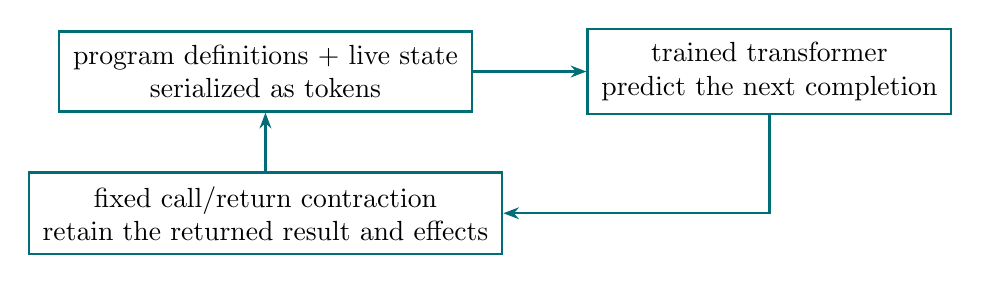
\begin{tikzpicture}
\node[box,minimum width=4.8cm] (state) at (0,0)
  {program definitions + live state\\serialized as tokens};
\node[box,minimum width=3.7cm] (model) at (6.4,0)
  {trained transformer\\predict the next completion};
\node[box,minimum width=4.8cm] (rewrite) at (0,-1.8)
  {fixed call/return contraction\\retain the returned result and effects};
\draw[arr] (state)--(model);
\draw[arr] (model.south)|-(rewrite.east);
\draw[arr] (rewrite)--(state);
\end{tikzpicture}
\end{center}
The reported 59.5M-parameter model executes held-out programs for bit operations,
arithmetic, and SAT tasks. Training uses next-token prediction on interpreter traces.

\point{The model performs retrieval and rewriting. The scaffold manages call contraction.}
\micsource
\end{frame}

\begin{frame}{The execution state has four distinct components}
A fixed procedure table maps names to parameters and bodies:
\[
 \Delta(f)=((x_1,\ldots,x_k),e).
\]
For this program, an execution configuration is
\[
 \sigma=\cfg{H}{\rho}{e}{K}.
\]
\begin{tabular}{@{}ll@{}}
$H:\cO\times\cA\rightharpoonup\cO$ & heap: object attributes and their values\\[3pt]
$\rho:\cV\rightharpoonup\cO$ & local environment: variable bindings\\[3pt]
$e\in\mathrm{Expr}$ & expression currently being evaluated\\[3pt]
$K$ & continuation stack: what remains to do
\end{tabular}

Here $\cO,\cA,\cV$ are object, attribute, and variable names.
The maps and stack are finite.
\source{Lecture formalization of MicroPy's semantic state. We inline expression
definitions; the paper stores them under separate expression names.}
\end{frame}

\begin{frame}{MicroPy's primitive operations}
\small
\begin{tabular}{@{}p{.39\textwidth}p{.57\textwidth}@{}}
\toprule
Expression & Effect of evaluation\\
\midrule
$\op{IF}(e_1,e_2,e_3)$ & Evaluate $e_1$; choose $e_2$ for $\true$, otherwise $e_3$.\\[4pt]
$\op{EQUAL}(e_1,e_2)$ & Test whether the resulting objects are identical.\\[4pt]
$\op{HasAttr}(e,a)$ & Test whether the resulting object has attribute $a$.\\[4pt]
$\op{LookupAttr}(e,a)$ & Read that attribute.\\[4pt]
$\op{Assert}(e_1,a,e_2)$ & Set the first object's attribute $a$ to the second value.\\[4pt]
$\op{SEQ}(e_1,e_2)$ & Evaluate $e_1$ for its effects, then return the value of $e_2$.\\[4pt]
$\op{Try}(e_1,e_2)$ & Try $e_1$; on $\fail$, roll back its writes and evaluate $e_2$.\\
\bottomrule
\end{tabular}

Also: object constants, $\op{LookupVar}(x)$, and $\op{App}(f,e_1,\ldots,e_k)$.
\source{Xu et al., Section 2.3. In our formalization, arguments are evaluated
left to right and a successful write returns $\unit$. Rollback rules are in backup.}
\end{frame}

\begin{frame}[fragile]{One procedure can flip a list of any finite length}
The heap represents a bit string by linked objects. The final object has no
\texttt{next} attribute.
\begin{center}
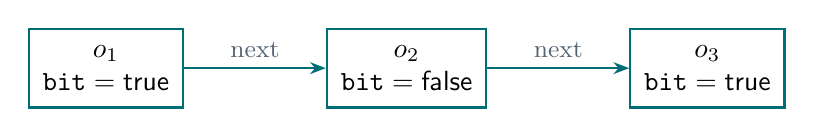
\begin{tikzpicture}[node distance=18mm]
\node[box] (a) {$o_1$\\$\mathtt{bit}=\true$};
\node[box,right=of a] (b) {$o_2$\\$\mathtt{bit}=\false$};
\node[box,right=of b] (c) {$o_3$\\$\mathtt{bit}=\true$};
\draw[arr] (a)--node[above,smalllabel]{next}(b);
\draw[arr] (b)--node[above,smalllabel]{next}(c);
\end{tikzpicture}
\end{center}
\begin{lstlisting}
def flip(x):
    x.bit = IF(x.bit, false, true)
    if HasAttr(x, next):
        return flip(x.next)
    else:
        return unit
\end{lstlisting}
\source{Readable surface notation for the lecture's MicroPy program;
the exact primitive expression is in backup.}
\end{frame}

\begin{frame}{One iteration: retrieve, choose, write, recurse}
Start with $\rho(x)=o_1$ and
$H(o_1,\mathtt{bit})=\true$.
\[
\begin{aligned}
 \op{LookupVar}(x)&\longmapsto o_1,\\
 \op{LookupAttr}(o_1,\mathtt{bit})&\longmapsto\true,\\
 \op{IF}(\true,\false,\true)&\longmapsto\false,\\
 \op{Assert}(o_1,\mathtt{bit},\false)
  &\longmapsto\unit,
  \qquad H'=H[(o_1,\mathtt{bit})\mapsto\false].
\end{aligned}
\]
Since $H'(o_1,\mathtt{next})=o_2$, the next call is $\mathtt{flip}(o_2)$.

\point{A longer list repeats the same rule types with different bindings.}
The next lookup must still find the correct object and its current value.
\end{frame}

\begin{frame}{A procedure call creates a new environment}
Suppose $\Delta(f)=((x_1,\ldots,x_k),e_f)$ and the arguments have evaluated
to objects $o_1,\ldots,o_k$. Write $\longmapsto^*$ for zero or more steps.
\[
\begin{split}
 &\cfg{H}{\rho}{\op{App}(f,o_1,\ldots,o_k)}{K}\\
 &\qquad\longmapsto^*
 \cfg{H}{[x_1\mapsto o_1,\ldots,x_k\mapsto o_k]}{e_f}
       {\op{Return}(\rho)::K}.
\end{split}
\]
When the body returns $o$ with heap $H'$:
\[
 \cfg{H'}{\rho_f}{o}{\op{Return}(\rho)::K}
 \longmapsto \cfg{H'}{\rho}{o}{K}.
\]
\point{Restore the caller's bindings; preserve the procedure's heap updates.}
The stack records the continuation. Recursion applies this same call rule again.
\source{An ordinary environment/continuation semantics for the lecture core.
MicroPy serializes these operations into several supervised rewrites.}
\end{frame}

\begin{frame}{The same variable name can have different bindings}
For $\Delta(\mathtt{id})=(x,\op{LookupVar}(x))$, call $\mathtt{id}(o_1)$
from an environment where $x$ denotes $o_0$.
\begin{center}
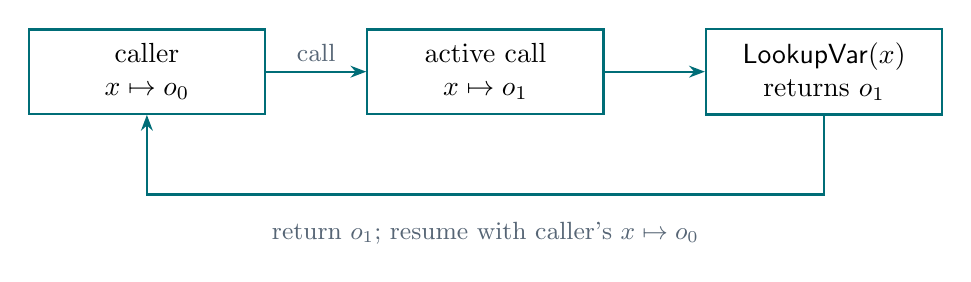
\begin{tikzpicture}
\node[box,minimum width=3cm] (outer) at (0,0) {caller\\$x\mapsto o_0$};
\node[box,minimum width=3cm] (inner) at (4.3,0) {active call\\$x\mapsto o_1$};
\node[box,minimum width=3cm] (lookup) at (8.6,0) {$\op{LookupVar}(x)$\\returns $o_1$};
\draw[arr] (outer)--node[above,smalllabel]{call}(inner);
\draw[arr] (inner)--(lookup);
\draw[arr] (lookup.south)--++(0,-1)-|(outer.south);
\node[smalllabel] at (4.3,-2.05)
  {return $o_1$; resume with caller's $x\mapsto o_0$};
\end{tikzpicture}
\end{center}
\vspace{5mm}
\point{Retrieval must respect scope, not just match the name \texttt{x}.}
Attribute retrieval must likewise select the latest applicable write to $(o,a)$.
\end{frame}

\begin{frame}{PENCIL deletes a completed subcomputation}
Once a call has produced its returned payload $\gamma$, apply
\[
 \underbrace{\alpha}_{\text{retained context}}\;
 \call\;
 \underbrace{\beta}_{\text{completed work}}\;
 \rightarrow\;
 \underbrace{\gamma}_{\text{result and effects}}\;\ret
 \quad\longmapsto\quad \alpha\,\gamma.
\]
The matching active call frame is removed. The payload includes the value
and any heap changes needed by the continuation.

\begin{center}
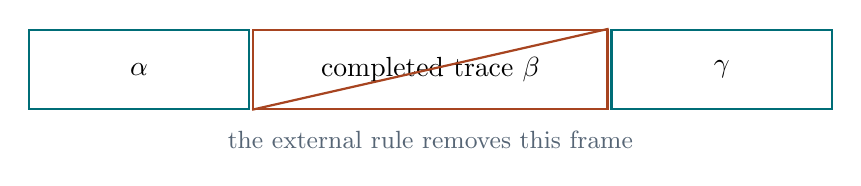
\begin{tikzpicture}
\node[box,minimum width=2.8cm] (a) at (0,0) {$\alpha$};
\node[box,draw=warm,minimum width=4.5cm] (b) at (3.7,0) {completed trace $\beta$};
\node[box,minimum width=2.8cm] (g) at (7.4,0) {$\gamma$};
\draw[warm,thick] (b.south west)--(b.north east);
\node[smalllabel] at (3.7,-.9) {the external rule removes this frame};
\end{tikzpicture}
\end{center}
\point{Keep the information needed to continue; reclaim the intermediate work.}
\source{PENCIL contraction as used by Xu et al., Equation (1).}
\end{frame}

\begin{frame}{Execution time and active memory can grow differently}
Let $L$ count execution steps, and let $S$ be the largest live configuration
size, including definitions, heap, and active calls.

\begin{columns}[T,onlytextwidth]
\begin{column}{.47\textwidth}
\textbf{Retain the complete transcript}

Every step contributes tokens. Even a loop over a small state keeps
increasing the context.
\[
 \text{retained history grows with }L.
\]
\end{column}
\begin{column}{.47\textwidth}
\textbf{Retain the live configuration}

Completed calls release their frames. A tail call can replace the current
frame instead of adding one.
\[
 \text{required state is governed by }S.
\]
\end{column}
\end{columns}
\point{For a list traversal, the list must remain available; old work need not.}
PENCIL provides the contraction mechanism. The returned state representation
determines how much memory is actually reclaimed.
\end{frame}

\begin{frame}{Fixed context bounds the interpreter's memory}
Suppose the entire persistent state is a string of at most $W$ tokens from
a vocabulary of size $V$. Each next call depends only on this string.
There are at most $N_W=\sum_{w=0}^{W}V^w$ persistent states.
\begin{proposition}[Finite-state execution]
Under deterministic decoding, a run with more than $N_W$ nonterminal states
repeats a state and then cycles forever.
\end{proposition}
\textbf{Proof.} Pigeonhole principle followed by determinism.

\point{At fixed context, this implementation is not a universal interpreter.}
PENCIL makes room for more execution steps by removing completed work.
Unbounded working memory still requires growing context and available objects.
\end{frame}

\begin{frame}{A finite rule set can have an unbounded input domain}
Schuurmans's controller always receives a prompt in the same 29-element set.
MicroPy's lookup rule must handle contexts containing increasingly many
bindings, scopes, positions, and intervening writes:
\[
 \op{LookupVar}(x)
 \quad\text{must retrieve the binding in the active call.}
\]
At context bound $W$, all token strings form a finite set of size $N_W$.
Increasing the memory bound increases this input domain.

\point{There is no fixed exhaustive input test as the allowed context grows.}
A correctness proof would need an argument that applies to every context size.
Learning can exploit the shared rules, but must generalize their retrieval
and rewriting to new structured inputs.
\end{frame}

\section{Learning and evidence}

\begin{frame}{Training data exposes the interpreter's intermediate work}
\begin{center}
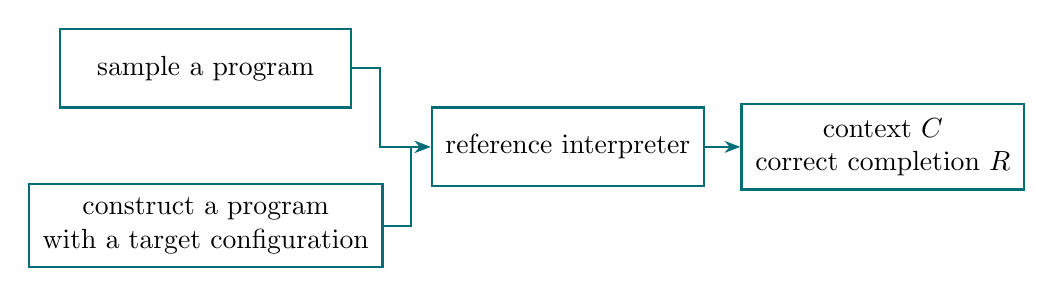
\begin{tikzpicture}
\node[box,minimum width=3.7cm] (prog) at (0,1) {sample a program};
\node[box,minimum width=3.7cm] (plan) at (0,-1) {construct a program\\with a target configuration};
\node[box,minimum width=3.1cm] (int) at (4.6,0) {reference interpreter};
\node[box,minimum width=3.2cm] (pair) at (8.6,0) {context $C$\\correct completion $R$};
\draw[arr] (prog.east)--++(.35,0)|-(int.west);
\draw[arr] (plan.east)--++(.35,0)|-(int.west);
\draw[arr] (int)--(pair);
\end{tikzpicture}
\end{center}
Random programs provide diverse executions. Targeted program generation exposes
rare cases: shadowed variables, intervening writes, and nested continuations.

\point{Choosing intermediate targets and their coverage is part of the method.}
\micsource
\end{frame}

\begin{frame}{The objective is ordinary next-token log loss}
For training pairs $(C_i,R_i)$, $i=1,\ldots,n$, minimize
\[
 \widehat L(\theta)
 =\frac1n\sum_{i=1}^n\sum_{j=1}^{|R_i|}
    -\log q_\theta(R_{i,j}\mid C_i,R_{i,<j}).
\]
$C_i$ is the observed interpreter context; $R_i$ is the reference completion.
Teacher forcing supplies its preceding tokens during training.

At execution time, generated tokens determine the next completion and hence
the next context after contraction.
\point{A short completion may require searching a large, structured context.}
The neural task includes locating the correct binding, not just choosing an
operation from a short list.
\end{frame}

\begin{frame}{The reported executions are substantially longer}
Training program executions are capped at \textbf{128 trace lines}.
The decoder-only transformer has \textbf{59.5 million parameters}.
\small
\begin{center}
\begin{tabular}{@{}lrrrr@{}}
\toprule
Test task & Instances & Max. lines & Max. context & Token accuracy\\
\midrule
Bit copying & 9 & 422 & 725 & 100\%\\
Bit flipping & 9 & 572 & 774 & 100\%\\
Binary addition & 9 & 2,365 & 1,514 & 100\%\\
Binary multiplication & 9 & 7,552 & 2,197 & 100\%\\
SAT solving & 180 & 5,020 & 2,091 & 100\%\\
SAT verification & 36 & 628 & 1,398 & 100\%\\
\bottomrule
\end{tabular}
\end{center}
\normalsize
252 test instances; 224,708 stepwise prompt/completion pairs.

{\color{accent}\bfseries $7{,}552/128\approx59$: familiar rules work in much longer runs.}
\source{Xu et al., Tables 1--2. Context is measured in tokens per step;
reported accuracy is token-level. Test sizes and metric details are in backup.}
\end{frame}

\begin{frame}{MicroPy generalizes over execution-trace length}
\begin{tabular}{@{}>{\raggedright\arraybackslash}p{.25\textwidth}
  >{\raggedright\arraybackslash}p{.33\textwidth}
  >{\raggedright\arraybackslash}p{.35\textwidth}@{}}
\toprule
Quantity & What increases? & What must generalize?\\
\midrule
Execution length $L$ & Number of interpreter steps & Repeated application of the learned rules\\[8pt]
Context length $W$ & Definitions, objects, live bindings and calls & Retrieval and rewriting with more live information\\[8pt]
Completion length $r$ & Tokens generated for one supervised step & Construction of a longer local response\\
\bottomrule
\end{tabular}

\point{The reported 59-fold increase concerns $L$.}
Test contexts reach 2,197 tokens. The paper gives no corresponding training
context-length range establishing extrapolation in $W$.
\source{Xu et al., Section 3 and Tables 1--2. Local completion-length
statistics are not reported.}
\end{frame}

\begin{frame}{Exact local prediction has a strong consequence}
Fix a deterministic decoder and the call/return protocol. Let
\[
 C_{t+1}=h(C_t,R_t),
\]
where $h$ appends completion $R_t$ and performs the prescribed contractions.
\begin{proposition}[Exact-prefix induction]
If the decoder predicts every token correctly on every reference prefix
of the required completions, including their stopping markers, then it
generates the entire reference execution exactly.
\end{proposition}
\textbf{Proof.} The first token agrees. Agreement through token $j-1$ gives
the reference prefix for token $j$. The completed response agrees, so $h$
produces the next reference context. Repeat.

\point{Literal zero errors is qualitatively stronger than a small average error.}
\end{frame}

\section{Self-contained neural interpreter}

\begin{frame}{Self-contained execution: one continuous generation}
Supply the program $p$ and input $x$. Ordinary autoregressive decoding produces
the execution and answer, without interpreter-specific external operations.

\textbf{With chain of thought (CoT):}
\[
 \enc(p,x)\ \longmapsto\
 \underbrace{r_1,\ldots,r_\ell}_{\text{intermediate tokens}}
 \ \longmapsto\ \enc(p(x)).
\]
The model must represent the evolving state and continue the computation
using its generated tokens.

\textbf{Direct output:}
\[
 \enc(p,x)\ \longmapsto\ \enc(p(x)).
\]
The answer tokens carry the output, with no separate intermediate trace.

\point{Self-contained describes execution. Training may still use execution traces.}
\end{frame}

\begin{frame}{Intermediate tokens provide additional computational time}
Let $d$ be transformer depth, $a$ the number of answer tokens, and $\ell$ the
number of intermediate tokens. At fixed input length, the sequential neural
depth available through decoding scales as
\[
\begin{array}{ll}
 \text{direct output:} & O(da),\\[5pt]
 \text{with CoT:} & O\bigl(d(\ell+a)\bigr).
\end{array}
\]
One continuous generation can therefore perform many successive computations.
Retaining its full transcript also makes the context grow with $\ell$.

\point{A short answer can require a long computation.}
Direct execution can exploit shortcuts for particular programs. A fixed-depth
model with a fixed short response has no adjustable execution-time budget.
CoT supplies one through the number of intermediate tokens.
\source{Computational-resource connection: Merrill and Sabharwal (2024),
\href{https://arxiv.org/abs/2310.07923}{The Expressive Power of Transformers
with Chain of Thought}. Formal complexity results return in later lectures.}
\end{frame}

\begin{frame}{The execution interface determines the tradeoffs}
\small
\begin{tabular}{@{}>{\raggedright\arraybackslash}p{.25\textwidth}
  >{\raggedright\arraybackslash}p{.34\textwidth}
  >{\raggedright\arraybackslash}p{.34\textwidth}@{}}
\toprule
Approach & What it provides & What it requires\\
\midrule
Controller with external memory &
Fixed neural context and a finite correctness test &
External code handles all memory addressing and updates.\\[8pt]
Scaffolded interpreter &
Learned structured retrieval and reclaiming completed work &
Live state fits in context. Retrieval must handle new configurations.\\[8pt]
Self-contained, with CoT &
Execution through ordinary generation, with adjustable time &
The model manages state in its trace. Retained context grows with that trace.\\[8pt]
Self-contained, direct output &
Short responses when the model can compute the answer directly &
The computation must fit the input-processing and output-generation budget.\\
\bottomrule
\end{tabular}
\normalsize
\point{Reducing external support transfers more of the execution to the learned model.}
\end{frame}

\begin{frame}{What these constructions teach us}
\textbf{Universality is a property of the whole system.}
A fixed neural controller can suffice when external memory grows.
MicroPy's context must grow to support unbounded live state.

\textbf{The learning problems differ.}
Schuurmans reduces neural correctness to a fixed finite table.
MicroPy learns retrieval and rewriting over structured contexts, and reports
generalization to longer execution traces.

\textbf{The more ambitious target is self-contained execution.}
The model carries out the computation through ordinary generation.
CoT provides intermediate steps. Direct output offers fewer steps when the
answer is short.

\point{Can we learn the execution rules and make them reliable as the required
time and memory grow?}
\end{frame}

\begin{frame}{Reading}
\textbf{Dale Schuurmans (2023).}\par
\emph{Memory Augmented Large Language Models are Computationally Universal.}\par
\href{https://arxiv.org/abs/2301.04589}{arXiv:2301.04589}\par
Sections 2--5: memory interface, universal machine, prompt program, finite test.

\medskip
\textbf{Ruize Xu, Chenxiao Yang, Yanhong Li, David McAllester (2026).}\par
\emph{Training Transformers as a Universal Computer.}\par
\href{https://arxiv.org/abs/2604.25166v1}{arXiv:2604.25166v1}\par
Section 2: execution model. Section 3: data and results.
Appendices B--D: concrete traces and definitions.

\source{The following backup slides provide the lecture's full core semantics,
proof details, and additional questions.}
\end{frame}

\appendix
\setbeamertemplate{footline}{\hfill\scriptsize Backup \insertframenumber\hspace{9mm}\vspace{3mm}}
\section{Backup material}

\begin{frame}{The universal machine used by Schuurmans}
Each entry is (written bit, head movement, next state).
\small
\begin{center}
\begin{tabular}{@{}cll@{}}
\toprule
State & Read 0 & Read 1\\
\midrule
$A$ & $(0,+1,B)$ & $(1,+1,A)$\\
$B$ & $(1,+1,C)$ & $(1,+1,A)$\\
$C$ & $(0,-1,G)$ & $(0,-1,E)$\\
$D$ & $(0,-1,F)$ & $(1,-1,E)$\\
$E$ & $(1,+1,A)$ & $(1,-1,D)$\\
$F$ & $(1,-1,D)$ & $(1,-1,D)$\\
$G$ & $(0,+1,H)$ & $(1,-1,G)$\\
$H$ & $(1,-1,I)$ & $(1,-1,G)$\\
\bottomrule
\end{tabular}
\hspace{12mm}
\begin{tabular}{@{}cll@{}}
\toprule
State & Read 0 & Read 1\\
\midrule
$I$ & $(0,+1,A)$ & $(1,-1,J)$\\
$J$ & $(1,-1,K)$ & $\halt$\\
$K$ & $(0,+1,L)$ & $(1,+1,N)$\\
$L$ & $(0,+1,M)$ & $(1,+1,L)$\\
$M$ & $(0,-1,B)$ & $(1,+1,L)$\\
$N$ & $(0,-1,C)$ & $(0,+1,O)$\\
$O$ & $(0,+1,N)$ & $(1,+1,N)$\\
\bottomrule
\end{tabular}
\end{center}
\normalsize
Blank $0$; initial state $A$. The tape encodes the program and its input.
State $F$ uses one prompt for both bits: 29 prompts for 30 state/bit pairs.
\source{Schuurmans, Table 1 and Section 4; machine attributed there to Neary and Woods.}
\end{frame}

\begin{frame}{Why the finite-table learning bound holds}
\begin{proposition}[Learning a finite table]
Draw $n$ independent labeled examples from $m$ possible inputs, each with
probability at least $p_{\min}>0$. If the fitted predictor agrees with all
observed labels, then its probability of an incorrect table is at most
$m e^{-np_{\min}}$.
\end{proposition}
\textbf{Proof.} If every input appears, consistency gives the correct table.
Writing $p_j$ for the probability of input $u_j$, the union bound gives
\[
\begin{aligned}
 \P(\text{an incorrect table})
 &\le\sum_{j=1}^m\P(u_j\text{ is absent})\\
 &=\sum_{j=1}^m(1-p_j)^n\le m e^{-np_{\min}}.
\end{aligned}
\]
Thus $n\ge \log(m/\eta)/p_{\min}$ suffices for failure probability at most $\eta$.
\end{frame}

\begin{frame}{The core language: syntax and conventions}
\small
Expressions have grammar
\[
\begin{aligned}
 e::={}&o\mid\op{LookupVar}(x)\mid\op{App}(f,e_1,\ldots,e_k)\\
 &\mid\op{IF}(e_1,e_2,e_3)\mid\op{EQUAL}(e_1,e_2)\\
 &\mid\op{HasAttr}(e,a)\mid\op{LookupAttr}(e,a)\\
 &\mid\op{Assert}(e_1,a,e_2)\mid\op{SEQ}(e_1,e_2)\mid\op{Try}(e_1,e_2).
\end{aligned}
\]
Objects include four distinct constants $\true,\false,\unit,\fail$.
Each procedure body has only its parameters as free variables; parameters are distinct.

We use left-to-right call-by-value evaluation. $\op{IF}$ evaluates only the
selected branch. A missing variable, procedure, or attribute is a stuck
configuration, not the explicit value $\fail$.

The semantics is deterministic on well-formed configurations. These choices
make a precise lecture core; the paper does not supply a complete executable
specification of all edge cases.
\end{frame}

\begin{frame}{A continuation records one unfinished operation}
\small
Let $K$ be a finite stack of frames, with $F::K$ placing $F$ on top.
\[
\begin{aligned}
 F::={}&\op{If}(e_2,e_3)\mid\op{Seq}(e_2)\mid\op{Try}(H_0,e_2)\\
 &\mid\op{EqL}(e_2)\mid\op{EqR}(o_1)\\
 &\mid\op{Has}(a)\mid\op{Get}(a)\\
 &\mid\op{SetL}(a,e_2)\mid\op{SetR}(o_1,a)\\
 &\mid\op{Args}(f,\bar o,\bar e)\mid\op{Return}(\rho_0).
\end{aligned}
\]
$\bar o$ contains evaluated arguments; $\bar e$ contains the remaining ones.
$\op{Return}(\rho_0)$ stores the caller's environment.

A terminal configuration is $\cfg{H}{\rho}{o}{[]}$.
We write $\sigma\longmapsto\sigma'$ for one transition and
$\longmapsto^*$ for zero or more transitions.
\point{The next rule depends on the active expression or on the top frame.}
\end{frame}

\begin{frame}{Core rules: lookup, conditionals, sequencing}
\small
In these rules, the procedure table is fixed and omitted.
\[
\begin{aligned}
 \cfg{H}{\rho}{\op{LookupVar}(x)}{K}
  &\longmapsto\cfg{H}{\rho}{\rho(x)}{K},\\[3pt]
 \cfg{H}{\rho}{\op{IF}(e_1,e_2,e_3)}{K}
  &\longmapsto\cfg{H}{\rho}{e_1}{\op{If}(e_2,e_3)::K},\\
 \cfg{H}{\rho}{\true}{\op{If}(e_2,e_3)::K}
  &\longmapsto\cfg{H}{\rho}{e_2}{K},\\
 \cfg{H}{\rho}{o}{\op{If}(e_2,e_3)::K}
  &\longmapsto\cfg{H}{\rho}{e_3}{K}\quad(o\ne\true),\\[3pt]
 \cfg{H}{\rho}{\op{SEQ}(e_1,e_2)}{K}
  &\longmapsto\cfg{H}{\rho}{e_1}{\op{Seq}(e_2)::K},\\
 \cfg{H}{\rho}{o}{\op{Seq}(e_2)::K}
  &\longmapsto\cfg{H}{\rho}{e_2}{K}.
\end{aligned}
\]
Each expression descends into the next required subexpression;
its frame determines how the returned object is used.
\end{frame}

\begin{frame}{Core rules: attribute reads and writes}
\small
\[
\begin{aligned}
 \cfg{H}{\rho}{\op{LookupAttr}(e,a)}{K}
  &\longmapsto\cfg{H}{\rho}{e}{\op{Get}(a)::K},\\
 \cfg{H}{\rho}{o}{\op{Get}(a)::K}
  &\longmapsto\cfg{H}{\rho}{H(o,a)}{K},\\[3pt]
 \cfg{H}{\rho}{\op{Assert}(e_1,a,e_2)}{K}
  &\longmapsto\cfg{H}{\rho}{e_1}{\op{SetL}(a,e_2)::K},\\
 \cfg{H}{\rho}{o_1}{\op{SetL}(a,e_2)::K}
  &\longmapsto\cfg{H}{\rho}{e_2}{\op{SetR}(o_1,a)::K},\\
 \cfg{H}{\rho}{o_2}{\op{SetR}(o_1,a)::K}
  &\longmapsto\cfg{H[(o_1,a)\mapsto o_2]}{\rho}{\unit}{K}.
\end{aligned}
\]
Writes replace the value of a heap entry. A serialized list of writes
implements this map by choosing the most recent matching entry.
\end{frame}

\begin{frame}{Core rules: tests}
\small
\[
\begin{aligned}
 \cfg{H}{\rho}{\op{HasAttr}(e,a)}{K}
  &\longmapsto\cfg{H}{\rho}{e}{\op{Has}(a)::K},\\
 \cfg{H}{\rho}{o}{\op{Has}(a)::K}
  &\longmapsto\cfg{H}{\rho}{b}{K},
\end{aligned}
\]
where $b=\true$ if $(o,a)\in\operatorname{dom}(H)$, and $b=\false$ otherwise.
\[
\begin{aligned}
 \cfg{H}{\rho}{\op{EQUAL}(e_1,e_2)}{K}
  &\longmapsto\cfg{H}{\rho}{e_1}{\op{EqL}(e_2)::K},\\
 \cfg{H}{\rho}{o_1}{\op{EqL}(e_2)::K}
  &\longmapsto\cfg{H}{\rho}{e_2}{\op{EqR}(o_1)::K},\\
 \cfg{H}{\rho}{o_2}{\op{EqR}(o_1)::K}
  &\longmapsto\cfg{H}{\rho}{b}{K},
\end{aligned}
\]
where $b=\true$ if $o_1=o_2$, and $b=\false$ otherwise.
\end{frame}

\begin{frame}{Core rules: evaluate arguments, then enter the body}
\small
For a nonempty argument list,
\[
\begin{split}
 \cfg{H}{\rho}{\op{App}(f,e_1,\ldots,e_k)}{K}
 \longmapsto\cfg{H}{\rho}{e_1}{\op{Args}(f,[],[e_2,\ldots,e_k])::K}.
\end{split}
\]
On returning an argument, either continue evaluating arguments,
\[
\begin{split}
 \cfg{H}{\rho}{o}{\op{Args}(f,\bar o,[e,\bar e])::K}
 \longmapsto\cfg{H}{\rho}{e}{\op{Args}(f,[\bar o,o],\bar e)::K},
\end{split}
\]
or enter the procedure. If $\Delta(f)=((x_1,\ldots,x_k),e_f)$, then
\[
\begin{split}
 &\cfg{H}{\rho}{o_k}{\op{Args}(f,[o_1,\ldots,o_{k-1}],[])::K}\\
 &\qquad\longmapsto
 \cfg{H}{[x_1\mapsto o_1,\ldots,x_k\mapsto o_k]}{e_f}{\op{Return}(\rho)::K}.
\end{split}
\]
A zero-argument call enters its body with the empty environment. A completed
body restores the environment stored by $\op{Return}$, as on the main call slide.
\source{The call transition in the main slides uses $\longmapsto^*$ to include these argument-collection steps.}
\end{frame}

\begin{frame}{Rollback preserves the state from before the attempted branch}
\small
\[
\begin{aligned}
 \cfg{H}{\rho}{\op{Try}(e_1,e_2)}{K}
 &\longmapsto\cfg{H}{\rho}{e_1}{\op{Try}(H,e_2)::K},\\
 \cfg{H'}{\rho}{\fail}{\op{Try}(H,e_2)::K}
 &\longmapsto\cfg{H}{\rho}{e_2}{K},\\
 \cfg{H'}{\rho}{o}{\op{Try}(H,e_2)::K}
 &\longmapsto\cfg{H'}{\rho}{o}{K}\quad(o\ne\fail).
\end{aligned}
\]
For example, start with $H(o,a)=\false$ and evaluate
\[
 \op{Try}\bigl(
   \op{SEQ}(\op{Assert}(o,a,\true),\fail),\
   \op{LookupAttr}(o,a)\bigr).
\]
The result is $\false$, and the final heap still satisfies $H(o,a)=\false$.
\point{The continuation needs both the fallback expression and the saved heap.}
\end{frame}

\begin{frame}{The bit-flipping example in the core language}
Write $v=\op{LookupVar}(x)$. The body of $\mathtt{flip}(x)$ is
\[
\begin{split}
 \op{SEQ}\bigl(&
 \op{Assert}(v,\mathtt{bit},
   \op{IF}(\op{LookupAttr}(v,\mathtt{bit}),\false,\true)),\\
 &\op{IF}(\op{HasAttr}(v,\mathtt{next}),
   \op{App}(\mathtt{flip},\op{LookupAttr}(v,\mathtt{next})),\unit)\bigr).
\end{split}
\]
\begin{proposition}[List traversal]
For a nonempty finite acyclic list with Boolean bit values, this program
terminates, returns $\unit$, flips each bit once, and leaves all other heap
entries unchanged.
\end{proposition}
\textbf{Proof.} Induct on list length. The write flips the first bit. For length
one there is no next attribute. Otherwise the next object starts the shorter
remaining list, and the recursive call has the claimed effect by induction.
\end{frame}

\begin{frame}{How the language can simulate a Turing machine}
Represent a sufficiently long finite tape segment by linked objects with
\texttt{left}, \texttt{right}, and \texttt{symbol} attributes.

Use one procedure $f_q(x)$ for each control state $q$. If
$\delta(q,b)=(b',+1,q')$, the corresponding branch performs
\[
 \op{SEQ}\bigl(\op{Assert}(x,\mathtt{symbol},b'),
             \op{App}(f_{q'},\op{LookupAttr}(x,\mathtt{right}))\bigr),
\]
where $x$ abbreviates its variable lookup. Use \texttt{left} for a left move;
the halting branch returns $\unit$.

\point{Every finite computation can be simulated with enough supplied tape objects.}
An unbounded simulation needs an unbounded supply of fresh cells, for example
through allocation. The reported experiments use supplied finite object memory.
\source{Lecture construction. Xu et al., Section 2.3, discuss preallocated heap
memory and an alternative allocating pairing primitive.}
\end{frame}

\begin{frame}{More distractors require a larger retrieval margin}
Suppose attention should retrieve one value, at position $j_*$. With scores
$s_j$ and inverse temperature $\beta>0$, its weight is
\[
 a_{j_*}=\frac{e^{\beta s_{j_*}}}{\sum_{j=1}^m e^{\beta s_j}}.
\]
If $s_{j_*}-s_j\ge\Delta>0$ for all $j\ne j_*$, then
\[
 a_{j_*}\ge\frac1{1+(m-1)e^{-\beta\Delta}}.
\]
For $m\ge2$ and $0<\varepsilon<1$, $a_{j_*}\ge1-\varepsilon$ is guaranteed when
\[
 \beta\Delta\ge\log\frac{(m-1)(1-\varepsilon)}{\varepsilon}.
\]
\point{Increasing the context can change the accuracy of a familiar retrieval rule.}
\end{frame}

\begin{frame}{What would a more informative length experiment measure?}
Hold the interpreter and decoding protocol fixed. Vary separately:

\begin{enumerate}
\item \textbf{Duration:} more iterations with similar live state size.
\item \textbf{Memory:} more objects and bindings at similar execution depth.
\item \textbf{Retrieval:} more distractors and greater distance to the relevant entry.
\item \textbf{Composition:} new nesting, variable shadowing, and write/read patterns.
\end{enumerate}

Measure exact completion accuracy and exact full-execution accuracy,
alongside token accuracy, and record the first error.

\point{These tests identify which shared rule stops transferring, and under what change.}
\end{frame}

\begin{frame}{Can execution introduce a new procedure name?}
The required state operation is simple:
\[
 \Delta_{t+1}=\Delta_t[f\mapsto((x_1,\ldots,x_k),e)].
\]
A later $\op{App}(f,o_1,\ldots,o_k)$ retrieves this body and uses the same
call rule as before.

\point{The new body belongs in writable program memory.}
In the reported MicroPy setup, procedure definitions are supplied in advance;
writes update object attributes.

A natural extension is to construct a body as data, bind it to a name, and
execute later calls. This adds a new learning question: can the model preserve
and use definitions created during the computation?
\end{frame}

\begin{frame}{A sign discrepancy in the printed Schuurmans program}
For state $G$ reading $0$, compare the specification with the printed code:
\[
\begin{array}{lll}
\text{Table 1} & \delta(G,0)=(0,+1,H) & \text{move right},\\[5pt]
\text{prompt }G & (0,-1,H) & \text{move left},\\[5pt]
\text{displayed response, test 12} & (0,-1,H) & \text{move left}.
\end{array}
\]
The displayed model response follows the prompt, but that prompt disagrees
with the stated Turing machine.

\point{The simulation theorem requires agreement with the transition table.}
Our construction uses Table 1. Matching the printed implementation to that
table requires correcting this sign and verifying the revised prompt.
\source{Schuurmans (2023): Table 1, Section 4's definition of $G$,
and Section 5's verification test 12.}
\end{frame}

\begin{frame}{Reading the empirical result precisely}
\small
\textbf{Test inputs.} The four bit tasks use lengths 2--10. SAT solving uses
2--4 variables and 1--6 clauses; SAT verification has 36 instances.

\textbf{Metric.} Tables 1--2 define accuracy as token-level success and report
100\% for each task. They do not provide raw token-error counts or a detailed
decoding protocol. Exact-prefix induction states the consequence of literal
zero errors under a fixed decoder and the same context protocol.

\textbf{Length.} The 128-line cap is stated for generator-sampled training
executions. Targeted plan sampling additionally supplies difficult local
configurations. No training-versus-test context-length distribution is given.

\textbf{Memory.} Live state and effects are serialized; PENCIL performs syntactic
contractions. The memory benefit depends on retaining a sufficient, compact
returned payload, including changes to mutable state.

\source{Xu et al., Sections 2--3, Tables 1--3, and Appendix B. These source
details are useful for interpreting and extending the experiment.}
\end{frame}

\end{document}
